\section{Implementation}
\subsection{Package structure}
Package structure decision was as important task in PokeMongo, we wanted to ensure an high level of readability and maintainability.
Although the classical “root package” which specifies the “domain.company.projet”, in our case “it.unipi.dii.lsmsd.pokemongo”, all the packages are structured \textit{by layers}. In this way, we decided to name the packages according to they function architecturally rather than their identity according to the business domain. Here the structure: 

\begin{figure}[H]
	\centering
	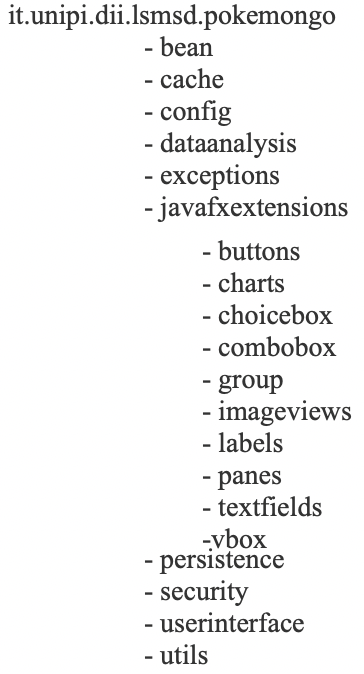
\includegraphics[width= 0.3\textwidth]{img/package_structure.png}
	\caption{Package Structure}
\end{figure}

We tried to maintain the name of the packages as simple as possible, and in a way they are all easy to read and to understand.
We also followed the convention of having the first character in the package names in lower case, in order to avoid conflicts with class or interface names.

\subsubsection{Package Analysis: Bean}
The “bean” package contains few classes that are used as beans while the application runs.

\begin{figure}[H]
	\centering
	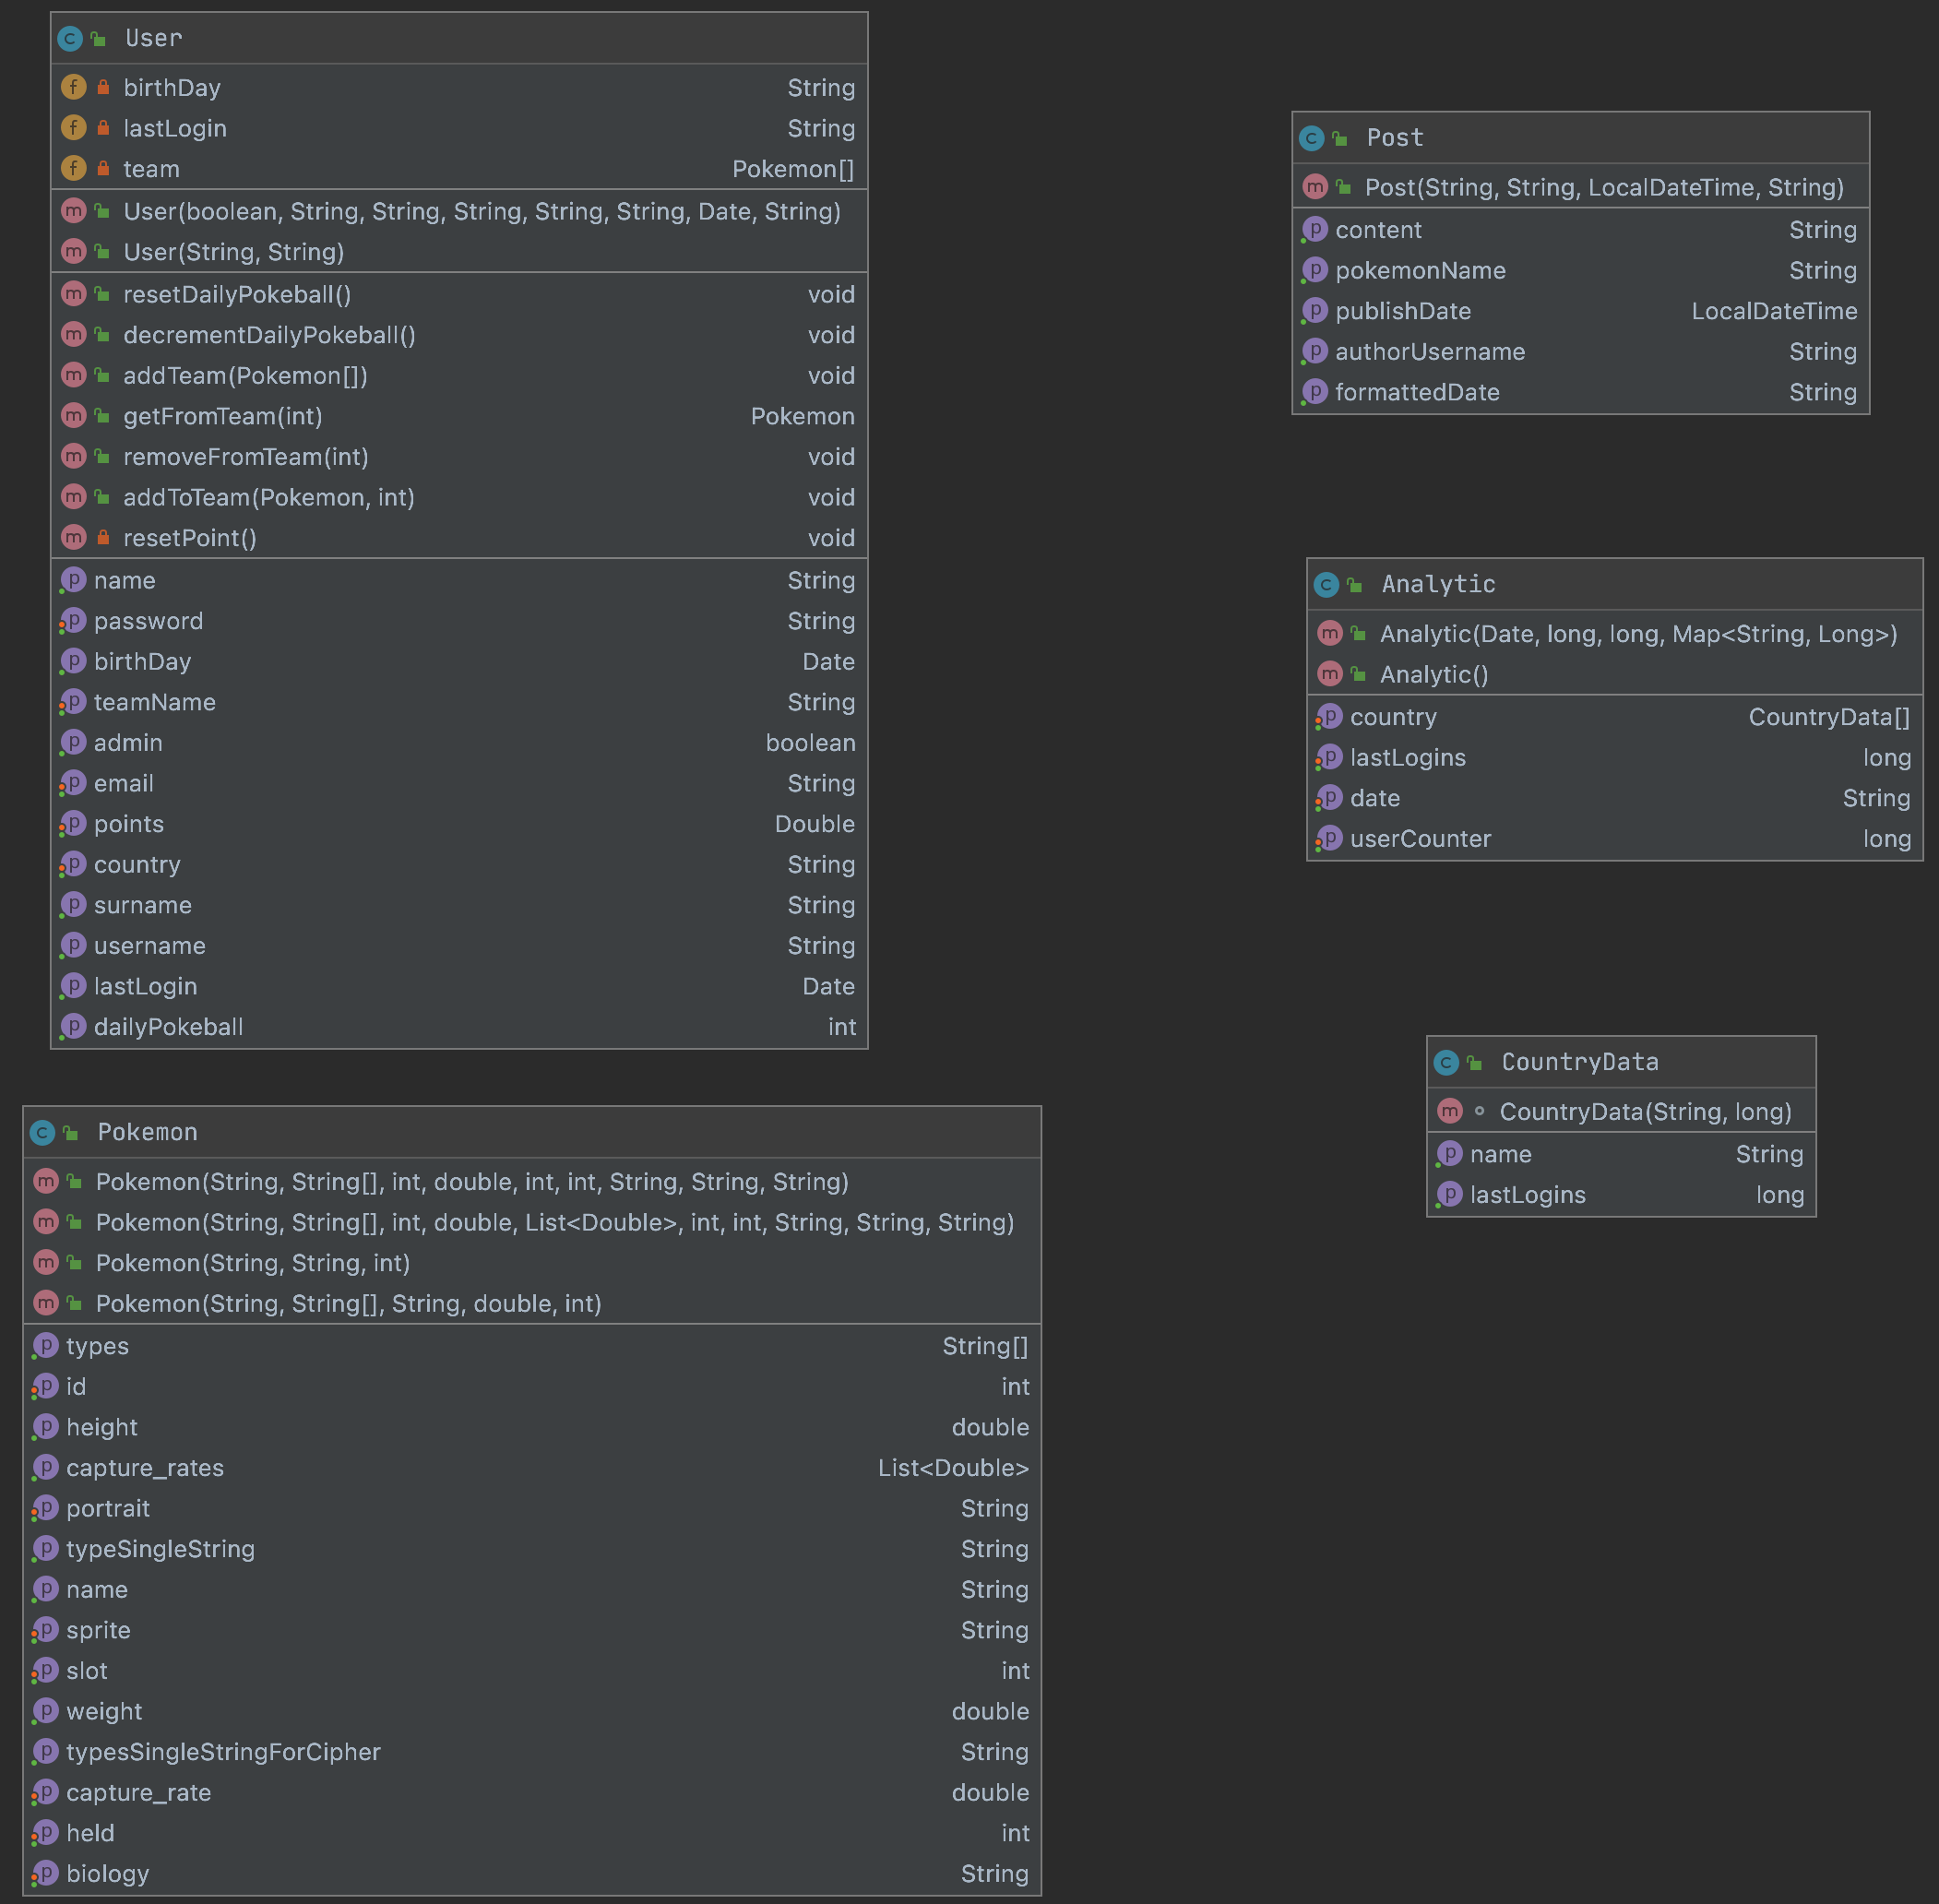
\includegraphics[width=0.9\textwidth]{img/bean_package.png}
	\caption{Bean Package Class Structure}
\end{figure}

\begin{center}
	\begin{tabular}{| m{9em} | m{22em} |} 
		\hline
		\textbf{Class Name} & \textbf{Short Description} \\ [0.5ex] 
		\hline
		User & The User class is used for instantiating object that refers to a specific user\\ 
		\hline
		Pokemon & The Pokemon class is used for instantiating object that refers to a specific Pokemon\\
		\hline
		Post & The Post class is used for instantiating object that refers to a specific Post. Responses (aka subPosts) are considered post also.\\
		\hline
		Analytic & This class is used for containing the information regarding a particular day.\\
		\hline
		CountryData & Used in the Analytic bean, it contains the information regarding a single country and the analytic strictly associated to it.\\
		\hline
	\end{tabular}
\end{center}

\subsubsection{Package Analysis: Cache}
The cache package contains classes that are helpful for caching images, we will talk about that in chapter 4.3.2. Despite what written above, this is one of the few packages that has a feature logic structure inside. We maintain in this package not only the classes/interface that handle the caching functionality, but also a javafx class extension which is PokemonImage. This class is strictly connected to the caching systems, because it contains the image we want to cache. We decided to use this approach to have a cleaner look and an easier maintainability for the caching systems. 
\begin{figure}[H]
	\centering
	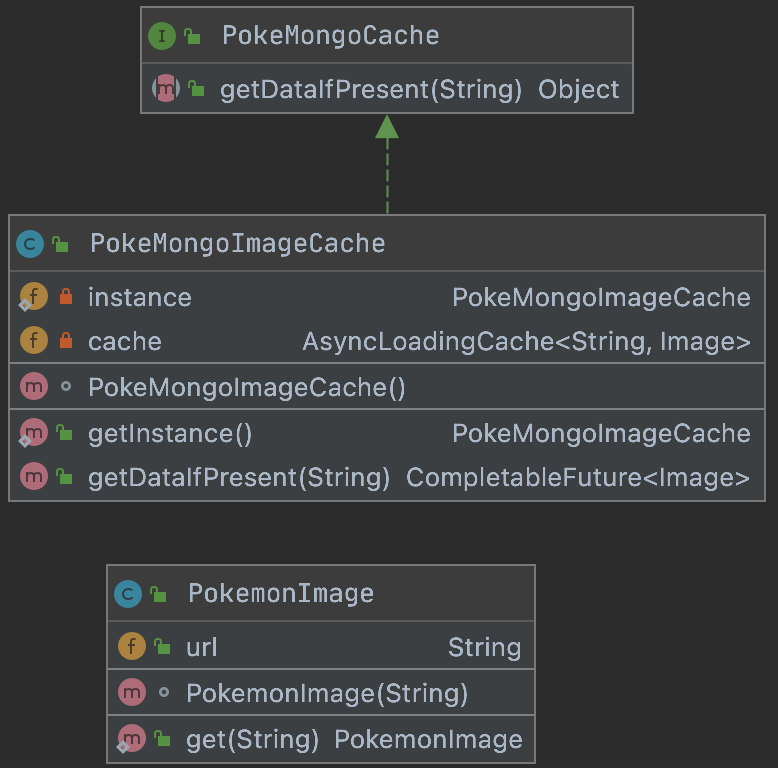
\includegraphics[width=0.4\textwidth]{img/cache_package.png}
	\caption{Cache Package Class Structure}
\end{figure}

\begin{center}
	\begin{tabular}{| m{14em} | m{19em} |} 
		\hline
		\textbf{Class Name} & \textbf{Short Description} \\ [0.5ex] 
		\hline
		PokeMongoCache & Simply an interface.\\ 
		\hline
		PokeMongoImageCache & The implementation of the interface described.\\ 
		\hline
		PokemonImage & An Image (javaFX) extension that will contains the image we want to show to the user in the GUI.\\ 
		\hline
	\end{tabular}
\end{center}

\subsubsection{Package Analysis: Cache}
This package is used for instantiating factory structures about the data analysis we made in the project. Every factory is dependent of an interface. 


\subsubsection{Packaging strategy and information hiding}
\subsubsection{UML package diagram}


\subsection{APIs and SPIs}

\subsection{Main tools}
\subsubsection{GSON}
\subsubsection{Caching mechanism and multimedia management}
\subsubsection{Password Encryptor}
\subsubsection{Logger}

\subsection{Analytics queries}
\subsubsection{User Rankings}
\subsubsection{Pokémon Rankings}
\subsubsection{Usage Statistics}
\subsubsection{Dynamic Catch Rate}


\subsection{Business logic}
\subsubsection{Points computing}
\subsubsection{Dynamic Catch Rate Computing}


